\section{Historie}

\begin{wrapfigure}{r}{5cm}

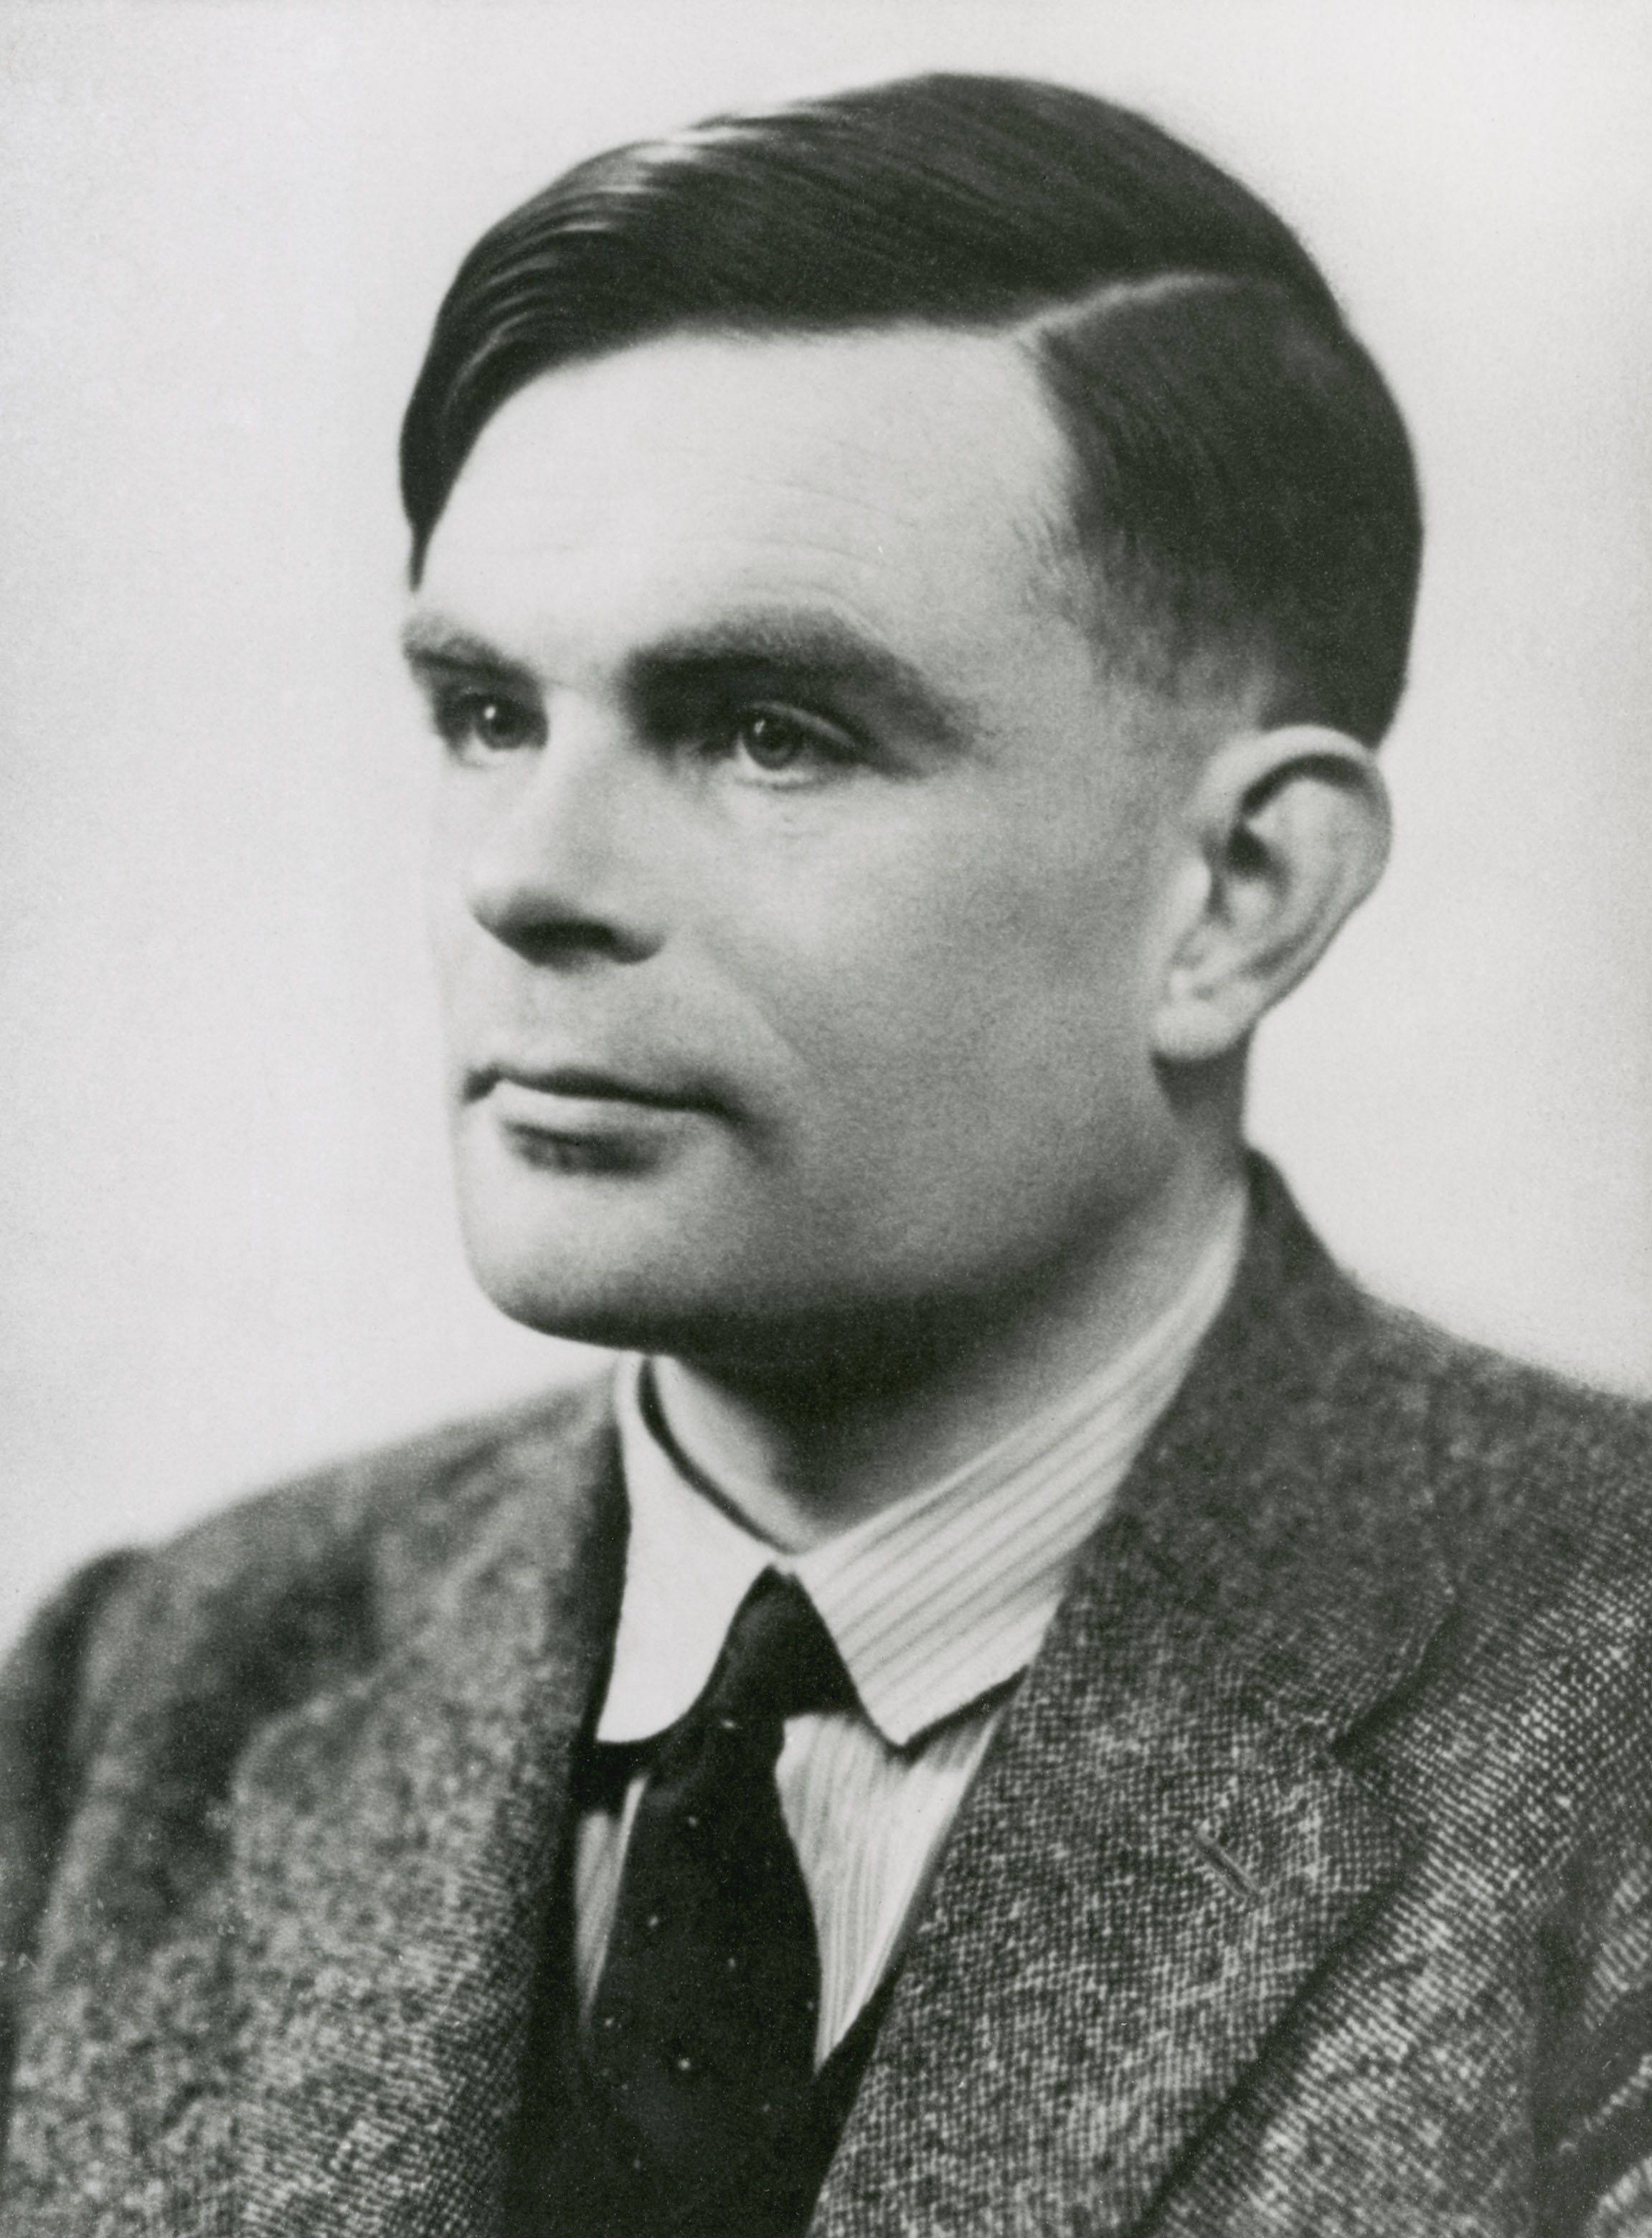
\includegraphics[scale=0.3]{Alan_Turing_Portrait.jpg}
\caption{Alan Turing}
\label{fig:turing}
\end{wrapfigure}

Alan Mathison Turing wurde 1912, am 23 Juni in London geboren.\\
Er machte seinen Abschluss an der Sherborne School in Dorset und besuchte anschließend ab Oktober 1931 das King's College in Cambridge, an dem er Mathematik studierte. Er beendete sein Studium 1934 und im März 1935 arbeitete er im Alter von 22 Jahren bereits als Dozent am King's College.\\
1936 veröffentlichte er eine seiner wichtigsten Werke "On Computable Numbers, with an Application to the Entscheidungsproblem", welche das Prinzip der Turing Maschine beinhaltet. Durch die Unterstützung von John von Neumann und Max Newman arbeiteten bereits mehrere Gruppen 1945 an der Umsetzung der Turing Maschine, also an der Umsetzung des ersten Computers. Turing verließ 1936 Cambridge um seine Forschungen an der Princeton University weiter zu führen und veröffentlichte 1938 "Systems of Logic Based on Ordinals".\\ 
Im Sommer 1938 kehrte Turing als Dozent an die King's zurück bis er beim Ausbruch des Krieges im September 1938 in den Bletchley Park zog, ein millitärisches Lager zur Entschlüsselung deutscher Nachrichten. Turings exzellente Arbeit hatte Kriegsentscheidente Konsequenzen. Turing war Hauptentwickler der Turing Bombe, einer extrem schnellen Entschlüsselungsmaschine. Im Nachhinein wird vermutet das die Arbeiten von Turing und seinen Kollegen den Krieg in Europa um mindestens 2 Jahre verkürzt hat.\\
Als der Krieg 1945 beendet war, ging Turing nach London ins National Physical Laboratory um seine Theorie der Turing Maschine in eine funktionierende Hardware umzusetzen. Im Februar 1947 veröffentlichte er "Lecture on the Automatic Computing Engine" in der er als Erster über Computerintelligenz schreibt und in seinem technischer Bericht 1948 "Intelligence Machinery" definiert er den Begriff 'Artificial Intelligence' kurz auch 'AI'. Im zwei Jahre später erschienenen Artikel "Computing Machinery and Intelligence" behandelt er den heute bekannten Turing Test, der testet ob ein System und die Intelligenz eines Menschen zu vergleichen ist.
Der erste Computer wurde im Juni 1948, auf Grundlage der Turing Maschine, am Computing Machine Laboratory, unter der Leitung von Max Newman, an der University of Manchester entwickelt. Noch im selben Jahr kam Turing der Einladung von Newman nach und wurde Direktor am Computing Machine Laboratory an der University of Manchester.\\
Turing wurde im März 1951, aufgrund seines großen Einflusses auf den Krieg, als Mitglied der Königlichen Gesellschaft erwählt.
Genau ein Jahr später, im März 1952 wird Turing in Manchester für seine Homosexualität, die in Britannien damals eine Straftat darstellte, mit einer zwölfmonatigen Hormontherapie zur Rechenschaft gezogen, die ihn Kastrierte. Turing erkrankte anschließend an einer Depression.\\
In den folgenden Jahren beschäftigte sich Turing mit künstlichem Leben und veröffentlichte 1952 den Artikel "The Chemical Basis of Morphgenesis", 1953 dann einen Artikel über Computerschach und schließlich in 1954 den Artikel "Solvable and Unsolvable Numbers" der sich auf einen früheren Artikel bezieht "On Computable Numbers".\\
Während weiterer Forschungen verstarb Turing schließlich unerwartet am 7 Juni 1954 im Alter von 41 Jahren an seinem Wohnort in Wilmslow in Cheshire. Es wird davon ausgegangen, dass Turing aufgrund seiner Depressionen Selbstmord begangen hat und sich mit dem Zyanid selbst vergiftete. Man kann aber nicht ganz ausschließen, dass Turing entweder durch Zyanid Dämpfe seiner Experimente oder auch durchaus durch einen Attentat ums Leben kam. 

